\documentclass[11pt]{article}
\usepackage{varnernotes}

\begin{document}

\lecturenotes{3a}{Equity Markets and the Stylized Facts of Growth Rates}{Fall 2026}{September 8, 2026}{Jeffrey D. Varner}

\learningobjectives
  {Describe equity claims}
  {Explain what common stock represents and distinguish the corporation, an exchange, an index, and an exchange-traded fund.}
  {Compute growth rates}
  {Calculate continuously compounded growth rates and convert them to log returns using $r=(\Delta t)g$.}
  {Diagnose stylized facts}
  {Use empirical distributions, autocorrelation, and conditional-volatility evidence to challenge an equity-return model.}

\section{Why Corporations Sell Ownership Claims}

Large ventures often require more capital and a longer horizon than one owner can supply. The joint-stock form separates the corporation from any single investor and divides the residual ownership claim into transferable shares. A common shareholder may receive voting rights and dividends, but stands behind contractual creditors in liquidation. Limited liability ordinarily caps the shareholder's loss at the invested amount; it does not protect the share price from falling to zero.

An \emph{equity security} is therefore a residual claim on a corporation, not a promise of fixed repayment. Its value depends on uncertain future distributions and resale opportunities. The market price aggregates heterogeneous beliefs, constraints, information, and orders into one executable quotation at a particular time.

An exchange supplies listing and trading rules and an organized venue for matching orders. Clearing and settlement complete the obligations created by trades, often through specialized infrastructure distinct from the matching engine. A stock index, such as the S\&P 500, is a rule-based numerical portfolio benchmark; it cannot itself be purchased. An exchange-traded fund (ETF) is a security whose shares trade intraday and whose portfolio may seek to track an index. These objects interact, but they are not interchangeable.

\section{Growth Rates and Returns}

A price change in dollars depends on the initial share price. We use the continuously compounded growth rate as the primary reward variable and reserve $r$ for the dimensionless log return over a specified interval.

\begin{definition}{Growth rate and log return}{return-measures}
Let $S_{t-1}>0$ and $S_t>0$ be consecutive share prices separated by $\Delta t>0$ years. The continuously compounded growth rate $g_t$ and corresponding log return $r_t$ are
\begin{equation}
  \label{eq:return-measures}
  g_t:=\frac{1}{\Delta t}\log\!\left(\frac{S_t}{S_{t-1}}\right),
  \qquad
  r_t:=(\Delta t)g_t=\log\!\left(\frac{S_t}{S_{t-1}}\right).
\end{equation}
Thus $g_t$ has units inverse years and $r_t$ is dimensionless. If dividends are included, use a consistently adjusted total-return price series before applying the definition.
\end{definition}

The choice between price and total return is substantive. A price-only series omits dividends, while an adjusted-price vendor may incorporate dividends and splits through its own convention. Data transformations must be documented before statistical conclusions are compared.

Log returns add across nonoverlapping time intervals (\propref{log-additivity}); equivalently, cumulative log return is a time-weighted sum of growth rates.

\begin{proposition}{Aggregation of price log returns}{log-additivity}
Let $S_0,S_1,\ldots,S_T$ be strictly positive prices and let $\Delta t_t$ be the length of interval $t$. Define $g_t:=(1/\Delta t_t)\log(S_t/S_{t-1})$ and $r_t:=(\Delta t_t)g_t$. Then
\begin{equation}
  \label{eq:log-additivity}
  \sum_{t=1}^{T}r_t
  =\sum_{t=1}^{T}(\Delta t_t)g_t
  =\log\!\left(\frac{S_T}{S_0}\right),
\end{equation}
which is the course convention $r=(\Delta t)g$ applied interval by interval.
\end{proposition}

\begin{derivation}
Use the logarithm of a product and cancel the intermediate price ratios:
\begin{equation*}
  \sum_{t=1}^{T}\log\!\left(\frac{S_t}{S_{t-1}}\right)
  =\log\!\left(\prod_{t=1}^{T}\frac{S_t}{S_{t-1}}\right)
  =\log\!\left(\frac{S_T}{S_0}\right).
\end{equation*}
The result is exact; the common approximation $\log(1+R_t)\approx R_t$ is only local for small $\lvert R_t\rvert$.
\end{derivation}

An excess growth rate compares the equity with a benchmark rate over the same interval. If $g_{f,t}$ is the benchmark growth rate, then $\bar g_t:=g_t-g_{f,t}$ and the corresponding excess log return is $\bar r_t=(\Delta t)\bar g_t$.

\section{Reward, Risk, and the Measurement Horizon}

The sample mean estimates average return under a chosen sampling rule; the sample standard deviation measures dispersion around that sample mean. Neither statistic alone describes downside magnitude, tail probability, drawdown, or liquidity. Moreover, annualizing daily volatility by multiplying by the square root of the number of periods relies on assumptions about scaling and dependence that empirical data may violate.

\begin{figure}[ht]
  \centering
  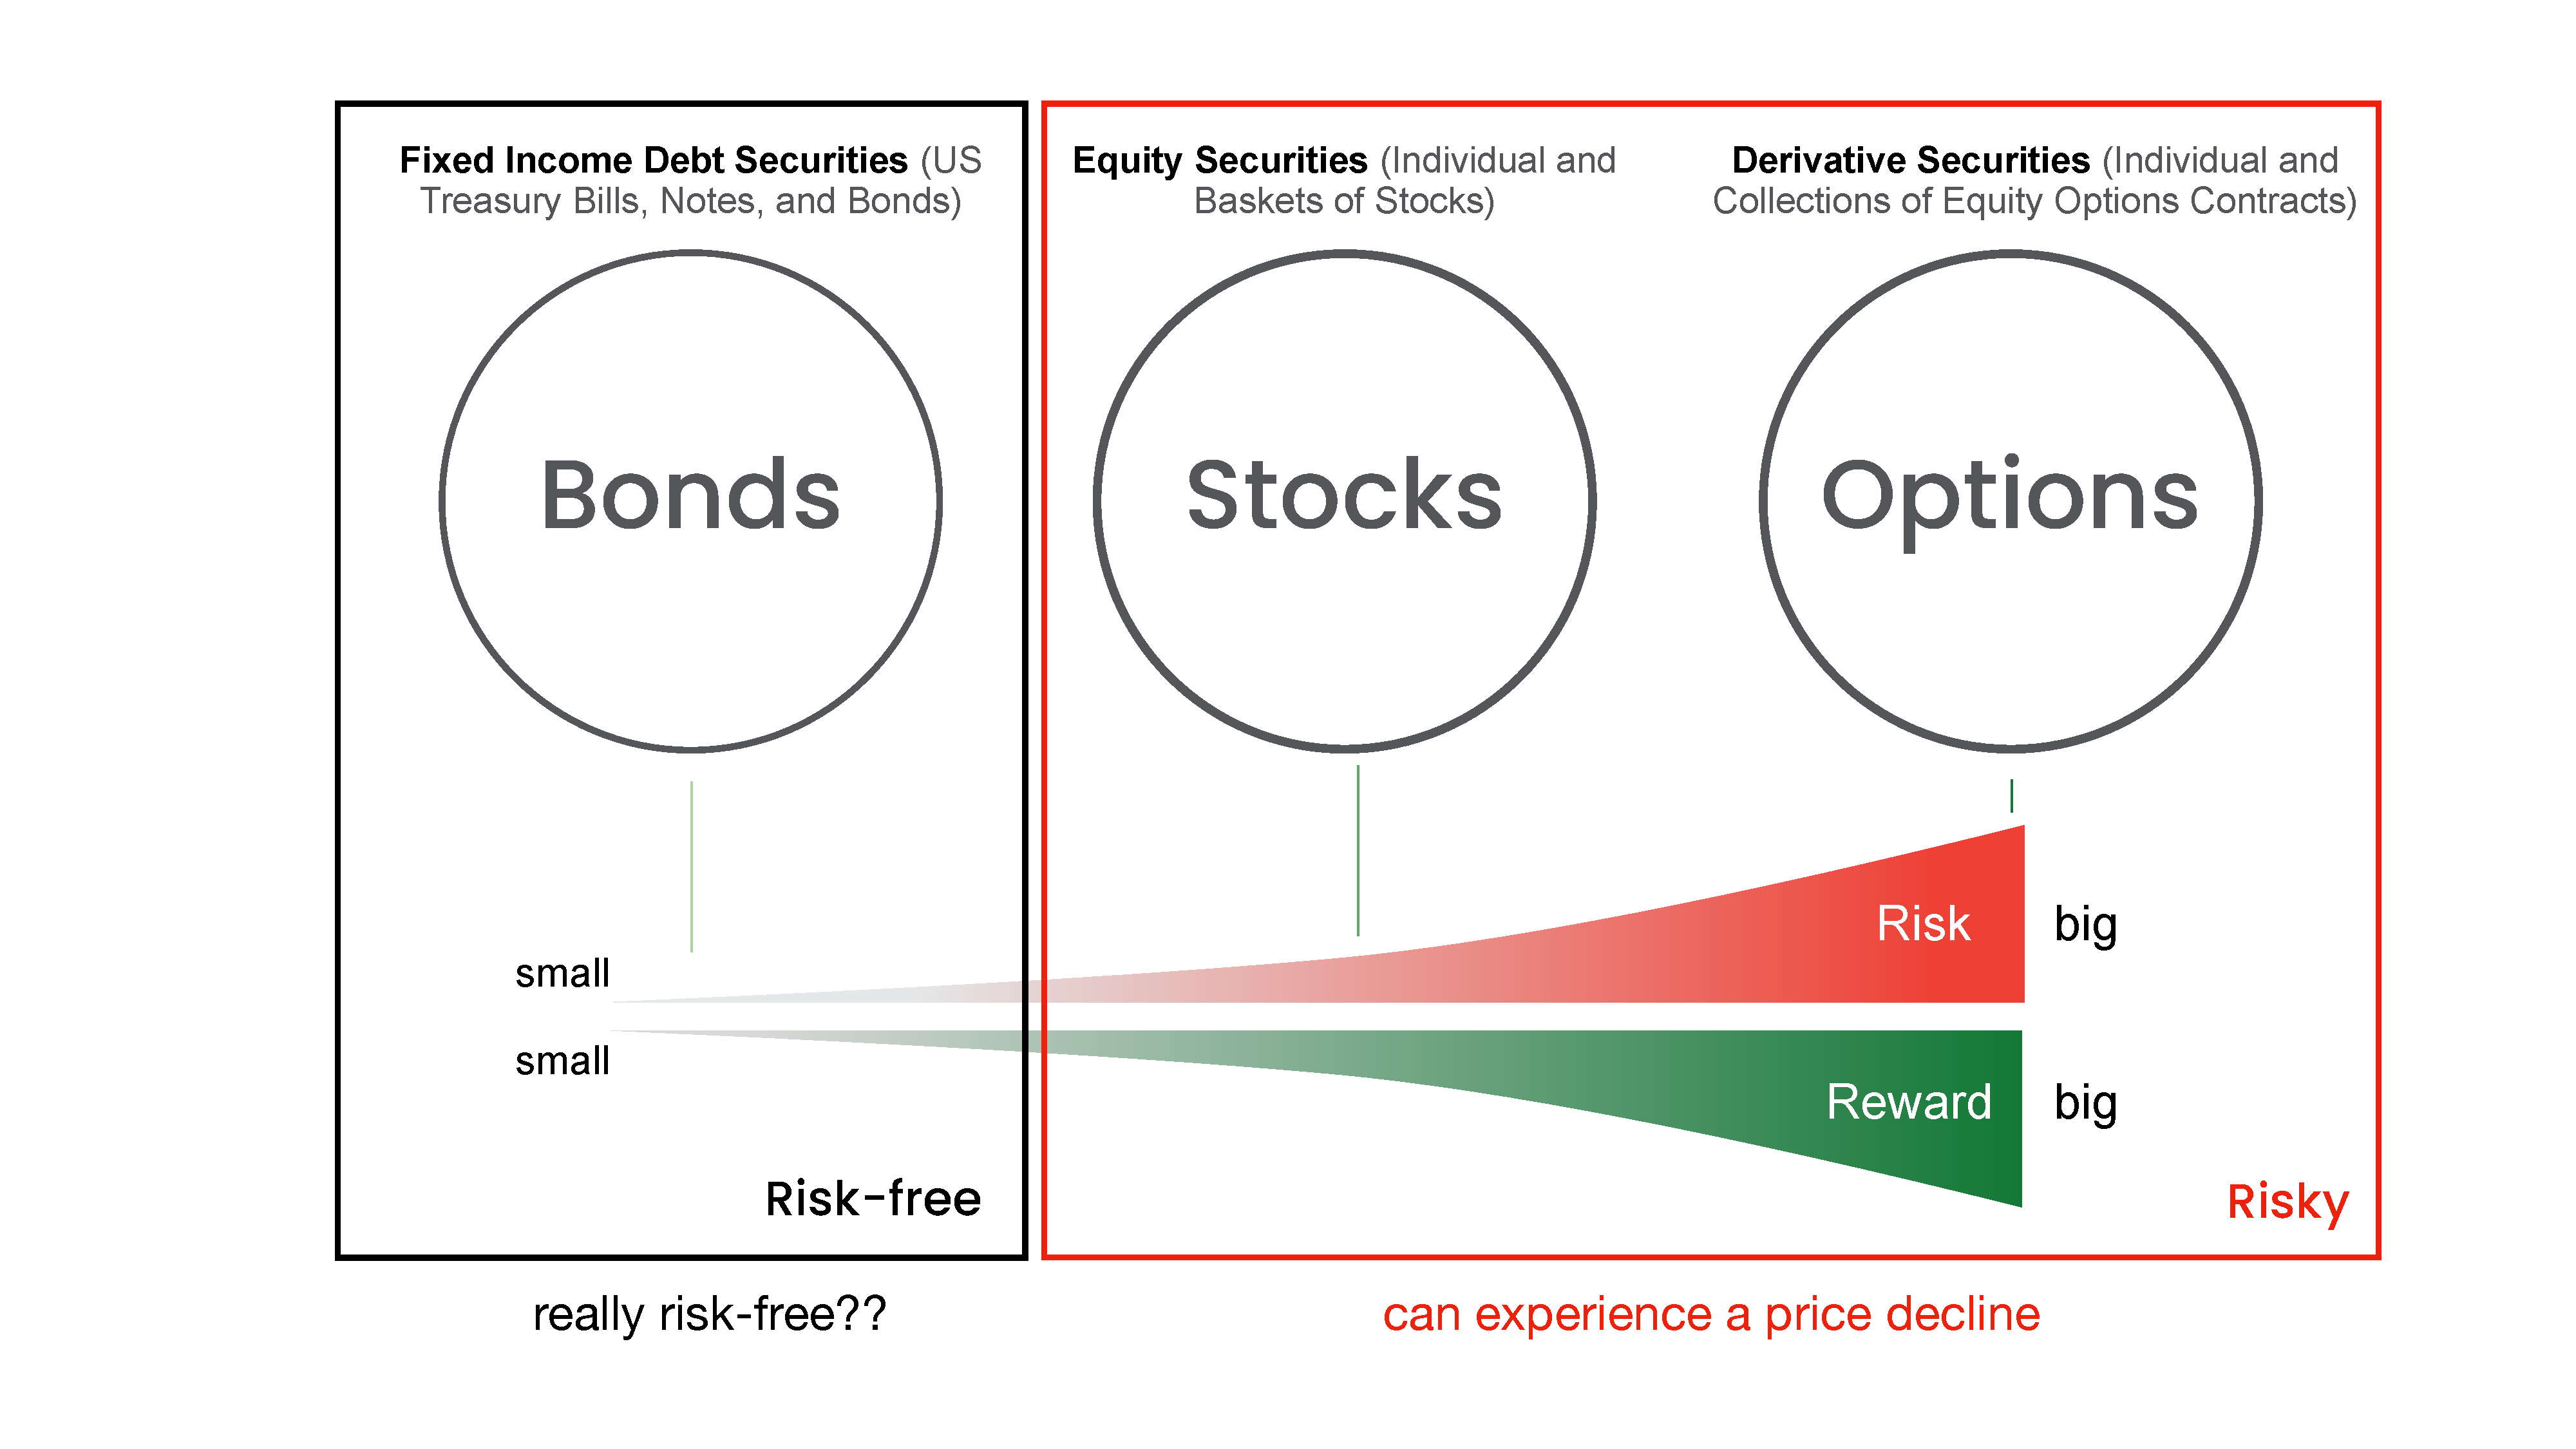
\includegraphics[width=0.72\textwidth]{../figs/Fig-RiskReward-Asset-Schematic.pdf}
  \caption{A conceptual risk--reward map. Expected reward and measured dispersion summarize different dimensions of an uncertain asset; assets with similar means and standard deviations can still have very different tail behavior, drawdowns, and liquidity.}
  \label{fig:risk-reward}
\end{figure}

The engineering question is not simply ``how volatile is this asset?'' It is ``which loss mechanism matters for this decision, over which horizon, and is the selected statistic sensitive to it?'' Value at risk, expected shortfall, maximum drawdown, downside deviation, beta, and tracking error each answer different questions.

\section{Stylized Facts as Model Requirements}

A stylized fact is a recurring empirical pattern observed across many assets or markets. It is not an exact law for every ticker and every sample. Stylized facts constrain useful models: a model that structurally cannot generate an important observed pattern should not be trusted for questions driven by that pattern.

\textbf{Heavy tails.}\enspace Large-magnitude returns occur more frequently than a fitted Gaussian model predicts. Sample kurtosis, quantile comparisons, tail plots, and tests such as Anderson--Darling can reveal distributional mismatch, but tail-index estimation is sensitive to the threshold and sample size. ``Heavy-tailed'' should be supported by a stated mathematical or empirical criterion rather than used as a synonym for volatile.

\textbf{Weak linear autocorrelation of raw returns.}\enspace At ordinary liquid-market horizons, signed returns often show small linear autocorrelations. This does not establish independence: nonlinear dependence, market microstructure effects, and conditional predictability can remain. Statistical significance also depends on the sample length and simultaneous testing across lags.

\textbf{Volatility clustering.}\enspace Large absolute or squared returns tend to occur near other large movements, and calm observations near other calm observations. The signed return may have little autocorrelation while $\lvert g_t\rvert$ or $g_t^2$ remains strongly dependent. Volatility is therefore conditional and time-varying rather than a fixed property revealed by one unconditional standard deviation.

\begin{figure}[ht]
  \centering
  \begin{tikzpicture}[x=0.58cm,y=0.72cm,>=Latex,font=\sffamily\footnotesize]
    \draw[vnink,line width=0.7pt,-{Latex[length=2.5mm]}] (0,0)--(18.2,0) node[right]{time};
    \draw[vnink,line width=0.7pt,-{Latex[length=2.5mm]}] (0,-2.25)--(0,2.25) node[above]{return};
    \draw[vnlink,line width=0.9pt]
      plot coordinates {(0.2,.1)(.6,-.2)(1,.15)(1.4,-.25)(1.8,.2)(2.2,-.1)(2.6,.18)(3,-.12)(3.4,.22)(3.8,-.18)(4.2,.1)(4.6,-.2)(5,.15)(5.4,-.12)(5.8,.25)(6.2,-.2)(6.6,.1)(7,-.15)(7.4,.2)(7.8,-.1)(8.2,.15)(8.6,-.25)(9,.2)(9.4,-.15)(9.8,.3)(10.2,-.55)(10.6,1.1)(11,-1.65)(11.4,.85)(11.8,-1.2)(12.2,1.8)(12.6,-.9)(13,1.25)(13.4,-1.55)(13.8,.7)(14.2,-.45)(14.6,.35)(15,-.25)(15.4,.2)(15.8,-.3)(16.2,.15)(16.6,-.2)(17,.1)(17.4,-.15)};
    \draw[vnrule,dashed] (9.6,-2)--(9.6,2);
    \draw[vnrule,dashed] (14.5,-2)--(14.5,2);
    \node[text=vnmuted,fill=white] at (12.05,2.0) {high-volatility cluster};
  \end{tikzpicture}
  \caption{A schematic return path with changing conditional dispersion. The high-volatility interval contains both positive and negative observations, so clustering concerns return magnitude rather than a persistent return sign.}
  \label{fig:volatility-clustering}
\end{figure}

The empirical notebook calculates these diagnostics for common stocks and ETFs. Its role is model criticism: the output should be compared with the assumptions and implications of the models introduced in L3b and L3b.

\notebooklink
  {L3a: Stylized Facts of Stocks and ETFs}
  {https://github.com/varnerlab/CHEME-5660-CourseRepository-Fall-2026/blob/main/lectures/week-3/L3a/CHEME-5660-L3a-StylizedFacts-Example-Fall-2026.ipynb}
  {Compare Normal, Laplace, and Student-$t$ fits; inspect Hill tail-index stability; and contrast signed-return with magnitude autocorrelation.}

\section{Many Assets Share Common Modes}

For $m$ dates and $n$ assets, collect centered returns in a matrix $G\in\mathbb{R}^{m\times n}$. Its singular value decomposition $G=U\Sigma V^{\mathsf T}$ expresses the data as ordered rank-one modes. Large singular values identify directions explaining substantial squared variation, often including a broad market-like co-movement. SVD is descriptive linear algebra: a mode is not automatically a causal economic factor, and results depend on centering, scaling, missing-data treatment, and the selected universe.

\notebooklink
  {L3a: SVD of S\&P 500 Growth Rates}
  {https://github.com/varnerlab/CHEME-5660-CourseRepository-Fall-2026/blob/main/lectures/week-3/L3a/CHEME-5660-L3a-SVD-SP500-Example-Fall-2026.ipynb}
  {Construct a multi-asset growth-rate matrix and use singular values and singular vectors to study common market modes.}

\newpage
\thispagestyle{fancy}
\keytakeaways
  {In this lecture, we treated equity as a residual ownership claim, constructed consistent return measures, and used recurring empirical patterns to challenge models.}
  {Returns require conventions}
  {Price versus total return, sampling interval, corporate-action adjustment, and compounding must be stated before statistics are compared.}
  {Dependence hides beyond returns}
  {Small autocorrelation in signed returns does not imply independence; absolute and squared returns often reveal persistent conditional volatility.}
  {Stylized facts are validation targets}
  {Heavy tails and volatility clustering expose risks that a fixed-variance Gaussian or i.i.d. model can systematically understate.}
  {Next, build a binomial equity lattice and separate real-world probabilities used for forecasting from risk-neutral probabilities used for pricing.}

\begin{readinglist}
  \item Rama Cont, \href{https://doi.org/10.1080/713665670}{``Empirical Properties of Asset Returns: Stylized Facts and Statistical Issues,''} \emph{Quantitative Finance} 1(2), 223--236 (2001).
  \item Benoit Mandelbrot, \href{https://www.jstor.org/stable/2350970}{``The Variation of Certain Speculative Prices,''} \emph{Journal of Business} 36(4), 394--419 (1963), for the early challenge to Gaussian return models.
  \item U.S. Securities and Exchange Commission, \href{https://www.investor.gov/introduction-investing/investing-basics/investment-products/stocks}{\emph{Stocks}}, for a concise description of shareholder claims and risks.
\end{readinglist}

\vfill
{\sffamily\footnotesize\color{vnmuted}\textbf{Educational use and risk notice.} These notes are for instruction only and do not constitute investment advice. Financial decisions involve risk, and model outputs depend on assumptions.}

\end{document}
